\documentclass[11pt, a4paper,english,spanish]{article}
\usepackage[spanish]{babel}
\usepackage[utf8]{inputenc}
\parskip = 11 pt
\usepackage[width=18cm, left=1.5cm, top=2.25cm, height= 25cm]{geometry}

\usepackage{amsmath}
\usepackage{amsfonts}
\usepackage{amssymb}
\usepackage{fancyhdr}
\usepackage{lastpage}
\usepackage{caratula}
\usepackage{url}
\usepackage{flafter}
\usepackage{afterpage}
\usepackage{float}
\usepackage{listings}
\usepackage{color}
\definecolor{gray97}{gray}{.97}
\definecolor{gray75}{gray}{.75}
\definecolor{gray45}{gray}{.45}
 
\usepackage{listings}
\lstset{ frame=Ltb,
     framerule=0pt,
     aboveskip=0.5cm,
     framextopmargin=3pt,
     framexbottommargin=3pt,
     framexleftmargin=0.4cm,
     framesep=0pt,
     rulesep=.4pt,
     backgroundcolor=\color{gray97},
     rulesepcolor=\color{black},
     %
     stringstyle=\ttfamily,
     showstringspaces = false,
     basicstyle=\small\ttfamily,
     commentstyle=\color{gray45},
     keywordstyle=\bfseries,
     %
     numbers=left,
     numbersep=15pt,
     numberstyle=\tiny,
     numberfirstline = false,
     breaklines=true,
   }


% minimizar fragmentado de listados
\lstnewenvironment{listing}[1][]
   {\lstset{#1}\pagebreak[0]}{\pagebreak[0]}
 
\lstdefinestyle{consola}
   {basicstyle=\scriptsize\bf\ttfamily,
    backgroundcolor=\color{gray75},
   }
 
\lstdefinestyle{C++}
   {language=C++,
   }
 
\newcommand{\real}{\ensuremath{\mathbb{R}}}
\newcommand{\grad}{\hspace{-2mm}$\phantom{a}^{\circ}$}

\pagestyle{fancy}

\title{MotionCapture}

%Estilo para el encabezado
\fancyhead[LO, LE]{Métodos Numéricos}
\fancyhead[RO, RE]{2$^{do.}$ cuatrimestre de 2014}
\fancyhead[CO, CE]{}

\fancyfoot[CO, CE]{P\'agina \thepage\ de \pageref{LastPage}}

\begin{document}
%Estos son los parametros para la caratula
\materia{Métodos Numéricos}
\submateria{Trabajo Pr\'actico Nro. 1}
\titulo{Sanguijuelas}
\fecha{\today}
\integrante{Martin Carreiro}{45/10}{martin301290@gmail.com}
\integrante{Kevin Kujawski}{459/10}{kevinkuja@gmail.com}
\integrante{Juan Manuel Ort\'iz de Z\'arate}{403/10}{jmanuoz@gmail.com}
\maketitle
\newpage

%Pagina de titulo e indice
\thispagestyle{empty}

\tableofcontents

\newpage

\normalsize
\section{Resumen}

Los sitios web a medida que fueron creciendo en cantidad en la época de los 90's, complicó el acceso a ellos o a menos que alguien te comentara o a través de publicidades, era muy dificil conocerlos. Es por eso, que fue el auge de los buscadores que a partir de palabras claves, podrían devolverte sitios que existan que puedan llegar a responder tu pregunta o tener el contenido. Un primer problema de entrada, es que, como todo en la vida, la calidad de dicho contenido puede no ser el deseado y existan mejores. Durante este trabajo repasaremos 3 algoritmos conocidos de ranqueo de páginas web, y veremos los resultados y los compararemos. \\
Una vez que sepamos cómo funcionan y cómo ordenan y ubican en los resultados dichos algoritmos, intentaremos responder a la pregunta: cuáles son los pasos a seguir para poder mejorar tu sitio y que salga dado una red, con mejor puntaje que la competencia.

\newpage
\section{Introducci\'on te\'orica}

\subsection{Matriz Dispersa}
   Se define una matrix dispersa aquella a la que la mayoría de sus elementos son cero.

   $$ 
\begin{bmatrix}
       0    &      0    &   0       &   0           &   a_{04}    \\
       0    &   a_{11}  &   a_{12}  &   0           &   0    \\
       0    &      0    &   0       &   a_{23}      &   0    \\
       0    &      0    &   0       &   a_{33}      &   0    \\
  a_{40}    &      0    &   0       &   0           &   0    \\
\end{bmatrix} 
$$

\subsection{DOK vs CRS vs CSC}
    La matriz dispersa al tener la propiedad de tener muy pocos valores no$-$cero es conveniente solo guardar estos y asumir el resto como cero. Existen varias estructuras como Dictionary of Keys (dok), Compressed Sparse Row (CSR) o Compressed Sparse Column (CSC). En el desarrollo de este TP, utilizamos DOK por facilidad en el uso del mismo. Tanto CSR o CSC se basan en la estructura Yale y se diferencian en como guardan los mismos valores, uno priorizando las columnas y otro las filas respectivamente.\\
    La estructura Yale consiste en a partir de la matriz original obtener tres vectores que contengan 
    \begin{itemize}
        \item A = los elementos no$-$cero de arriba-abajo,izquierda-derecha
        \item IA = los indices para cada fila i del primer elemento no-cero de dicha fila
        \item JA = los indices de columna para cada valor de A
    \end{itemize}
    Si bien en caso de que haya en una fila muchos números no-ceros es más beneficioso la utilización de esta estructura, la facilidad con DOK permite hacer pruebas más rápido.
\newpage
\section{Desarrollo}

\subsection{Matriz Banda}

Como explicamos en la introducción de la matriz banda, llegamos a la conclusión de que la matriz de ecuaciones de la representación del parabrisas tenía forma de la denominada "matriz banda" cuya respectiva banda era de tamaño m+m+1 con m siendo el ancho del parabrisas. Este es un hecho importante ya que las matrices banda tienen caracteristicas especiales de las cuales es posible la optimización temporal y espacial para resolver el sistema de ecuaciones con eliminación gausseana.

\subsubsection{Optimización espacial}

El problema de representar la matriz original es que la mayoría de los valores son 0 y solo importan los elementos de la banda de la matriz, por lo tanto una forma de optimizar espacialmente es solo guardar la banda, con lo que se logra reducir considerablemente el espacio en esta representación, ya que suponiendo que se tiene un parabrisas de n filas y m columnas, el tamaño de la matriz original sería de $(n*m)^2$, mientras que con la optimización de matriz banda quedaría de tamaño (n*m)*(2*m+1).

El método para construir la representación optimizada de la matriz banda es simple, se guardar la diagonal en una matriz, quedando en el centro los elementos de la diagonal dependiendo de lo que haya en esa posición, ya que en el caso de que sea vacía esta deberá tener coeficientes de las posiciones adyacentes. Además nos dimos cuenta que se podía representar la matriz de tal forma que presente una mejor optimización temporal, y consiste en no poner los coeficientes de las celdas vacias adyacentes si estas no son vacias, en tal caso al vector de resultados le restamos la temperatura de la misma, generando que luego no sea necesario considerar las posiciones no vacias para la eliminación gausseana a la hora de resolver el sistema.

\begin{verbatim}

por cada posición del parabrisas //O(N*M)
       pos = fila posicion + columna posicion * ancho;
		
              si en esa posición hay una SANGUIJUELA:
			
                     bandMatrix[pos][ancho] = 1;
                     resultados[pos] = ts;
		
              si esa posición es borde FRIO:
                    
                     bandMatrix[pos][ancho] = 1;
                     resultados[pos] = -100;


              en caso de que esa posición sea VACIA:
                     bandMatrix[pos][ancho] = -4;
                     resultados[pos] = 0;
                    
                     si la izquierda no es vacìa
                            resultados[pos] -= temperatura del de la izquierda;
                     else
                             bandMatrix[pos][ancho-1] = 1;

                    si la de arriba no es vacìa
                            resultados[pos] -= temperatura del de arriba;
                     else 
                            bandMatrix[pos][0] = 1;

                     si la de la derecha no es vacìa
                            resultados[pos] -= temperatura del de la derecha;
                     else 
                            bandMatrix[pos][ancho+1] = 1;
                     
                     si la de abajo no es vacìa
                            resultados[pos] -= temperatura del de abajo;
                     else 
                            bandMatrix[pos][ancho*2] = 1;
		

\end{verbatim}
\subsubsection{Optimización temporal}

\subsubsection{Ejemplo}
\begin{figure}[htb]
\begin{center}
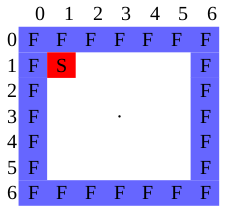
\includegraphics[scale=0.70]{imagenes/parabrisasej.png} 
\caption{Vista de la representación de Parabrisas del ejemplo} 
\end{center}
\end{figure}

\newpage
\begin{figure}[htb]
\begin{center}
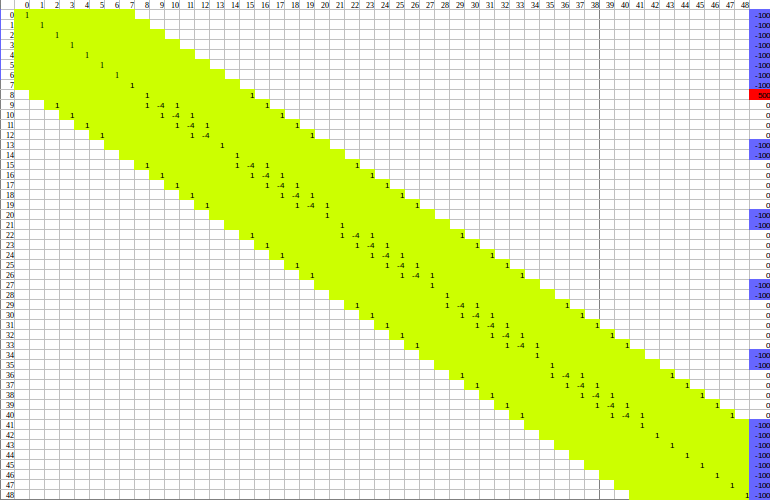
\includegraphics[scale=0.50]{imagenes/matrizej.png} 
\caption{Matriz de ecuaciones del ejemplo} 
\end{center}
\end{figure}

\newpage

\begin{figure}[htb]
\begin{center}
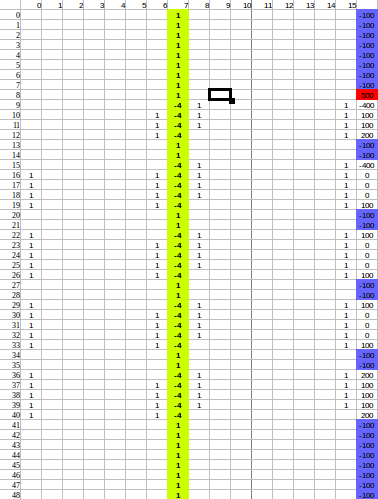
\includegraphics[scale=0.70]{imagenes/matrizbandaej.png} 
\caption{Matriz banda del ejemplo} 
\end{center}
\end{figure}

\newpage

\subsection{Soluciones}

Para resolver el problema que se nos pide, planteamos distintos tipos de solución. Inicialmente encaramos el problema de manera exacta, pero lo deshechamos inmediatamente ya que sabiendo que es un problema de decisión, el tiempo para determinar cuál es el número mínimo de sanguijuelas a eliminar es exponencial en la cantidad de estas. Es por eso que decidimos realizar una heurística, ya que el tiempo es preciado cuando el parabrisas de nuestra nave tiene poco tiempo antes de que se rompa en caso de estar en situación crítica. Para modo de comparación tomamos dos tipos de algoritmos para establecer que es una mejor solución.



seleccionar que sanguijuelas matar, pensamos una solución Greedy  (\ref{sec:MatrizCuadrada}) + Local Search . Esta consiste, a grandes rasgos, en ir matando las sanguijuelas del medio (ya que son las que mayor temperatura generan en el punto crìtico) hasta que el punto central este por debajo del 235 Cº. Para tener algún parámetro de referencia pensamos en buscar otra solución posible, y asì  compararlas y chequear que esta sea mejor. Esta solución alternativa consiste básicamente en seleccionar aleatoriamente que sanguijuelas aniquilar. Procederemos ahora a explicar en detalle las implementaciones de estas soluciones.

\subsection{Solución Greedy + Local Search}
Esta solución consiste, a grandes rasgos, en ir matando las sanguijuelas del medio (ya que son las que mayor temperatura generan en el punto crítico) hasta que el punto central este por debajo del 235 Cº. Finalmente, tratar de realizar una búsqueda local intentado volcar de vuelta en el parabrisas sanguijuelas que habíamos decidido sacar y viendo si era realmente necesario eliminarla para poder salir del estado crítico. La decisión de hacer LocalSearch está dada para el caso de que exista una sanguijuela en el centro y dos a la misma distancia. Pero de un lado haya una linea de muchas sanguijuelas, por lo que es muy probable que con sacar la del lado de la linea fuera suficiente.

Pseudocodigo:

\begin{verbatim}
Class Windshield{
    greedySolution(){
        orderLeachesByDistanceToCenter()
         while(!this->isCooledDown(){
             leachesToRemove(this->removeFirstNotRemovedLeachOrderedCentrically())
         }

         localSearchTryToReturnLeaches(leachesToRemove);

         return leachesToRemove;
    } 
    isCooledDown(){
         recalculateByBandMatrix();
         return (matrix.centerPoint < Ts)
    }
    orderLeachesByDistanceToCenter(){
        sort(leaches).by(lambda {|leach,otherLeach| leach.distanceToCenter < otherLeach.distanceToCenter})
    }

    localSearchTryToReturnLeaches(leachesToRemove){
        for (leach in leachesToRemove){
            putBackLeachInWindshield(leach);
            if (isCooledDown){
                leachesToRemove.erase(leach)
            }else{
                takeOutLeachFromWindshield(leach);
            }
        }
    }
}
\end{verbatim}



\subsection{Solución Random}\label{sec:solucionRandom}


En esta solución seleccionamos de nuestro array de posiciones de sanguijuelas (que es el array recibido por parametro, osea con las posiciones sin discretizar) una al azar y la eliminamos. Luego ejecutamos de nuevo el cálculo de las temperaturas y chequeamos si el punto crìtico esta por debajo del 235 Cº.Si no lo está, elegimos otra al azar y repetimos el proceso hasta que lo esté. 

Pseudocodigo:

\begin{verbatim}
Class Windshield{
    randomSolution(){
         while(!this->isCooledDown(){
             this->randomKill()
         }
    } 
    isCooledDown(){
         return (matrix.centerPoint < Ts)
    }
    randomKill(){
         randomRemove(posSanguijuelas)
         this->recalculateTemps()
    }
}
\end{verbatim}

Vale aclarar que el recalculateTemps utiliza el metodo band matrix, ya que este es màs rápido.










\newpage
\section{Experimentación Y Resultados}

A continuación expondremos los resultados obtenidos por cada algoritmo para distintas imágenes. El objetivo será posteriormente hacer análisis de calidad subjetiva (es decir que vemos a simple vista), objetiva y tiempo de computos. Para, como dijimos en un principio, determinar ventajas y desventajas de cada uno de ellos. Para los análisis objetivos desarrollamos un programa en python que compara pixel a pixel

TINCHER TERMINA DE EXPLICAR ACA QUE HACE EL PYTHON QUE COMPARA IMAGENES

\subsection{Colores}

Se nos ocurrió que podría ser interesante chequear los comportamientos de estos procedimientos en una imagen con muchos bordes ya que estos, en algoritmos como el directional, son factores importantes y potencialmente conflictivos. Además hicimos que la imagen sea grande (5000 x 3000 pixeles) para poder analizar tiempos de computo y para influir en la calidad subjetiva, ya que si ponemos imagenes con mucha definición pequeños errores podrían pasar desapercividos para el ojo humano.

Tambien expondremos la imagen bayerizada para que quede claro que la conversción que estamos haciendo es correcta.

\begin{figure}[!htb]

\minipage{0.5\textwidth}
\begin{center}
       
\includegraphics[scale=0.08]{imagenes/colores.png}
       \caption{Original }\label{fig:awesome_image1}
        \end{center}
\endminipage\hfill
\minipage{0.5\textwidth}
\begin{center}
        
\includegraphics[scale=0.08]{imagenes/colores_bayer.png}
       \caption{Bayerizada}\label{fig:awesome_image1}
        \end{center}
\endminipage\hfill 
\end{figure}
\newpage
\begin{figure}[!htb]
\minipage{0.5\textwidth}
\begin{center}
    
\includegraphics[scale=0.08]{imagenes/colores_demosicing_bilineal.png}
    \caption{Bilineal }
 \end{center}
\endminipage
\minipage{0.5\textwidth}
\begin{center}
    
\includegraphics[scale=0.08]{imagenes/colores_demosicing_quality.png}
    \caption{High Quality}
        \end{center}
\endminipage\hfill
\end{figure}
\newpage
\begin{figure}[!htb]
\minipage{0.5\textwidth}
\begin{center}
    
\includegraphics[scale=0.08]{imagenes/colores_demosicing_spline.png}
    \caption{Directional}
        \end{center}
\endminipage
\minipage{0.5\textwidth}
\begin{center}
    
\includegraphics[scale=0.08]{imagenes/colores_demosicing_vecino.png}
    \caption{Vecinos}
 \end{center}
\endminipage
 
\end{figure}
\newpage

Efectivamente a primera vista parecería que todas dieran lo mismo. Pero veamos que si le hacemos zoom, no es así.
\begin{figure}[!htb]
\minipage{0.5\textwidth}
\begin{center}
    
\includegraphics[scale=0.6]{imagenes/colores_bilineal_zoom.jpg}
    \caption{Bilineal Zoom}
        \end{center}
\endminipage
\minipage{0.5\textwidth}
\begin{center}
    
\includegraphics[scale=0.6]{imagenes/colores_hq_zoom.jpg}
    \caption{Bilineal Zoom}
        \end{center}
\endminipage 
\end{figure}
\begin{figure}[!htb]
\minipage{0.5\textwidth}
\begin{center}
    
\includegraphics[scale=0.6]{imagenes/colores_directional_zoom.jpg}
    \caption{Directional Zoom}
        \end{center}
\endminipage
\minipage{0.5\textwidth}
\begin{center}
    
\includegraphics[scale=0.6]{imagenes/colores_vecinos_zoom.jpg}
    \caption{Vecinos Zoom}
        \end{center}
\endminipage 
\end{figure}

Como supimos el algoritmo directional y el bilineal tuvieron pequeños errores en los bordes. Podemos observar que en esos casos entre el verde y el violeta parece haber como una `cosedura', la misma se repite en todos los bordes de la imagen. Estas diferencias imperceptibles por el tamaño de la imagen a primera vista pueden ser efectivamente comprobadas mediante un análisis de calidad objetivo. 

PSNR 41.14 con bilineal
PSNR 39.67 con quality
PSNR 48.13 con directional
PSNR 48.13 con vecinos

tiempos:




\newpage
\section{Discusi\'on}

\subsection{PageRank}
Claramente podemos notar que a medida que el C crece, el algoritmo toma más iteraciones en achicar la norma. Esto se debe a que el grado de aleatoriedad elimina el peso de la unión entre los sitios e indica una uniformidad en el comportamiento, entonces la matriz si bien estocástica ahora se encuentra distribuida esa suma $=$ 1 por columna en varias filas. Esto produce mayor cantidad de iteraciones en el método de la potencia ya que la mayor uniformidad de la matriz provoca que ninguna 'zona' de la matriz absorba más que las demás.   $[1]$\\
También es bastante notorio que a pesar de que los distintos casos de prueba sean muy diferentes entre si y hasta cientos de veces más grandes, la evolución de la norma converge de formas casi idénticas y lo mismo sucede para las iteraciones requeridas hasta llegar a la norma variando el parámetro c.



\subsection{HITS}
En todos los casos podemos observar que tanto el vector de hubs como el de autridades convergen de forma muy similar, sólo en la instancia grande hay una pequeña diferencia pero es bastante despreciable. 
Por otro lado podemos ver que los casos en los que mas drásitca es la convergencia (abortion y genetic) los valores inciales de la norma manhattan son muy altos (alrrededor de 100), provocando asi que se equiparen con las que comienzan en valores mas bajos pero convergen mas lentamente (movies y standford).
En estos dos últimos casos además podemos notar grandes saltos de convergencia pasando en pocas iteracion de 1$e^{20}$ a menos de 1$e^{80}$, entiendiendo, aca sí, que la diferencia es totalmente despreciable y el valor obtenido ya ha convergido. De todas formas consideramos que puede ser un punto de interés para analizar mas en profundidad ya que más allá de decir que entendemos de eso, no sabríamos explicar porque se produce ese salto. 

\subsection{Ejemplos de comportamiento esperado}

A continuación veremos en redes pequeñas como se comporta cada algoritmo para ver si su comportamiento es el esperado.

\subsubsection{HITS}
 \begin{figure}[!htb]
\begin{center}
    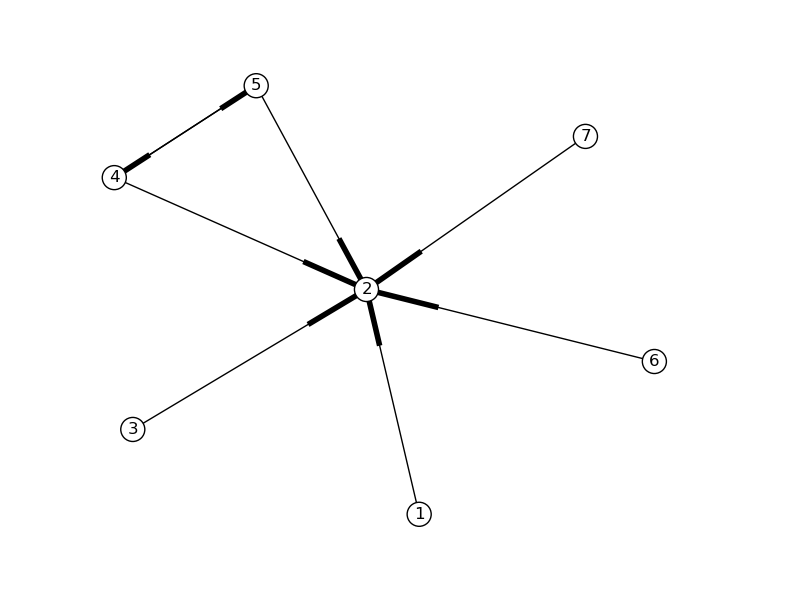
\includegraphics[scale=0.5]{imagenes/test4.png}
    \caption{Red de 7 nodos}
    \end{center}
\end{figure}

Resultado obtenido:
   $$ 
\begin{bmatrix}
              &    Autoridad  &  Hub \\
 Nodo 1 &   0.000000    &      0.383092       \\
 Nodo 2   &  0.967054    &  0.000000     \\
 Nodo 3   &  0.000000   &     0.383092  \\
 Nodo 4   &  0.180008    &     0.454401       \\
 Nodo 5   &  0.180008    &     0.454401        \\
 Nodo 6   &  0.000000    &      0.383092     \\
 Nodo 7   &  0.000000   &     0.383092 \\
\end{bmatrix} 
$$

Efectivamente podemos observar que en la columna de autoridades el nodo 2 es el mayor ya que es el que mas apuntado esta y todos aquellos que tienen 0 es porque no son apuntados por ninguno. Por otro lado en la columna de hubs podemos ver que los nodos 4 y 5 son los que mayor valor tienen ya que son los que mas apuntan a otros nodos con 2 salidas.

\subsection{Análisis cualitativo}

En esta sección procederemos a discutir sobre la calidad de resultados que obtenemos de cada algoritmo y luego los compararemos entre si.\\
Como el objetivo de este trabajo práctico esta enfocado al ranking web que se le asigna a los distintos sitios de internet, consideramos como buenos resultados aquellos que aparecerían en la primer página de los buscadores, es decir, los primero 10 resultados serán los que consideraremos para el análisis.

\subsubsection{PageRank}
Según el paper de Bryan y Leise, quienes proponen el algoritmo, lo más común es que el valor del navegante aleatorio sea de 0.15. Por lo tanto creemos que con este valor es donde aparecerán los mejores resultados, pero también veremos que sucede con valores de 0.5 y 0.85, ya que estos valores indican por un lado que la probabilidad del navegante entre quedarse e irse es equiprobable y por otro lado es el inverso de lo que ellos consideran como el valor más común. En valores de 0 y 1 no tendrían sentido el análisis ya que por un lado daría la matriz original y por el otro una matriz equiprobable.\\
El caso de prueba que utilizaremos es el dado por la cátedra, \textbf{Abortion}, y lo elegimos ya que es un tema bastante discutido donde se pueden encontrar resultados interesantes.


\paragraph{Resultados con un c=0.15}
\begin{enumerate}
\item
 \textbf{No relacionado con el tema}\\
http://www.allexperts.com/about.asp\\
AllExperts.com
\item
http://www.nrlc.org\\
National Right to Life Organization
\item
\textbf{No relacionado con el tema}\\
http://www.phone-soft.com/at/cyber-world/international/o1480i.htm\\
PHONE-SOFT INTERNET DIRECTORY INTERNATIONAL:HERB THERAPY LINKS
\item

http://www.lm.com/~jdehullu\\
Ariadne's Thread: On abortion, affirmative action, hate speech
\item


http://www.plannedparenthood.org\\
Planned Parenthood Federation of America
\item

http://www.gynpages.com\\
Abortion Clinics OnLine
\item

http://www.care-net.org/link.htm\\
CareNet Links
\item

http://www.naral.org\\
NARAL: Abortion and Reproductive Rights: Choice For Women
 \item

http://www.crosswalk.com/ftr/1,,17,00.htm \\
Crosswalk.com Forums - Welcome
 \item

http://www.cais.com/agm/main\\
The Abortion Rights Activist Home Page

\end{enumerate}

\paragraph{Resultados con un c=0.5}
 \begin{enumerate}
 \item http://www.allexperts.com/about.asp\\
AllExperts.com
 \item http://www.nrlc.org\\
National Right to Life Organization
 \item \textbf{No relacionado con el tema}\\
 http://home.about.com\\
About - The Human Internet
 \item \textbf{No relacionado con el tema}\\
http://www.phone-soft.com/at/cyber-world/international/o1480i.htm\\
PHONE-SOFT INTERNET DIRECTORY INTERNATIONAL:HERB THERAPY LINKS
 \item http://www.lm.com/~jdehullu\\
Ariadne's Thread: On abortion, affirmative action, hate speech
 \item http://www.plannedparenthood.org\\
Planned Parenthood Federation of America
 \item http://www.care-net.org/link.htm\\
CareNet Links
 \item http://www.gynpages.com\\
Abortion Clinics OnLine
 \item http://www.marchforlife.org\\
The March For Life Fund Home Page
 \item \textbf{No relacionado con el tema}\\
http://www.jbs.org\\
The John Birch Society
 \end{enumerate}
 
\paragraph{Resultados con un c=0.85}
 \begin{enumerate}

 \item 
 \textbf{No relacionado con el tema}\\
 http://www.jbs.org\\
The John Birch Society
 \item 
 \textbf{No relacionado con el tema}\\
http://home.about.com\\
About - The Human Internet
 \item 
 \textbf{No relacionado con el tema}\\
http://www.allexperts.com/about.asp\\
AllExperts.com
 \item
  \textbf{No relacionado con el tema}\\
http://www.aobs-store.com\\
American Opinion Book Services Online Store
 \item
http://www.nrlc.org\\
National Right to Life Organization
 \item 
 \textbf{No relacionado con el tema}\\
http://www.trimonline.org\\
TRIMonline - Lower Taxes Through Less Government
 \item
http://www.marchforlife.org\\
The March For Life Fund Home Page
 \item 
 \textbf{No relacionado con el tema}\\
http://www.phone-soft.com/at/cyber-world/international/o1480i.htm\\
PHONE-SOFT INTERNET DIRECTORY INTERNATIONAL:HERB THERAPY LINKS
 \item 
\textbf{No relacionado con el tema}\\
http://www.reagan.com\\
The Reagan Information Interchange
 \item 
 \textbf{No relacionado con el tema}\\
http://www.pregnancycenters.org\\
Pregnancy Centers Online
 \end{enumerate}

En base a los resultados se puede ver como a medida que aumenta el $c$ empiezan a aparecer resultados que poco tienen que ver con el tema directamente, ya que puede estar relacionado de alguna forma o no diferenciarse tanto del eje temático.\\
Nos pareció extraño que aparece siempre muy bien posicionado el sitio web All Experts, que nada tiene que ver con el tema de los abortos, por lo tanto decidimos hacer un foco especial en este para ver porque sucedía esto y llegamos a la conclusión que es debido a que el factor mas determinante es que gran cantidad de sitios referidos al tema y a su vez bien posicionados (aunque fuera del top 10) apuntaban al mismo, y por lo tanto le daban bastante peso a All Experts.\\
Sucede algo parecido con otro sitio de venta de software que aparece pero no nos pareció importante su análisis ya que es un claro caso de publicidad paga en anuncios de los sitios que hablan sobre el tema.\\
Aunque se pueda ver que con un $c$ menor los resultados tienen relación con el tema nos pareció que no son lo suficiente buenos como para considerarlos excelente resultados cuando se busca sobre un tema tan discutido como el aborto, esperando quizás más definiciones sobre el tema y luchas por su legalización/penalización. 

\subsubsection{HITS}

\subsubsection{Comparación}


\newpage
\section{Conclusiones}

En caso de una imagen con cambios grandes en zonas pequeñas, todos los algoritmos tienden a fallar en esas zonas.
Esto se debe a que todos los algoritmos dependen fuertemente de los pixeles próximos cercanos, los cuales poseen valores muy distintos al valor a calcular. Esto es denominado borde.

\newpage

\end{document}

